% CVPR 2022 Paper Template
% based on the CVPR template provided by Ming-Ming Cheng (https://github.com/MCG-NKU/CVPR_Template)
% modified and extended by Stefan Roth (stefan.roth@NOSPAMtu-darmstadt.de)

\documentclass[10pt,twocolumn,letterpaper]{article}

%%%%%%%%% PAPER TYPE - PLEASE UPDATE FOR FINAL VERSION

\usepackage{cvpr}
% Include other packages here, before hyperref.
\usepackage{graphicx}
\usepackage{amsmath}
\usepackage{amssymb}
\usepackage{booktabs}
\usepackage{multirow}
\usepackage{tabularx} % Add this to your preamble
\usepackage{array}    % Added: Needed for \newcolumntype
\usepackage{calc}
\usepackage[pagebackref,breaklinks,colorlinks]{hyperref}

% Define a new column type for centered 'X' columns for tabularx
\newcolumntype{C}{>{\centering\arraybackslash}X} % Added: Definition for C column type

% Support for easy cross-referencing
\usepackage[capitalize]{cleveref}
\crefname{section}{Sec.}{Secs.}
\Crefname{section}{Section}{Sections}
\Crefname{table}{Table}{Tables}
\crefname{table}{Tab.}{Tabs.}


%%%%%%%%% PAPER ID - PLEASE UPDATE
\def\cvprPaperID{*****} % *** Enter the CVPR Paper ID here
\def\confName{CVPR}
\def\confYear{2022}

%%%%%%%%%%%%%%%%%%%%%%%%%%%%%%%%%%%%%%%%%%%%%%%%

\begin{document}
	
	%%%%%%%%% TITLE
	\title{\textbf{From Query-Based Segment Retrieval to Answer Generation in Egocentric Videos}}
	
	
	
	\author{Arvin Esmaeily\\
		s324665\\
		\and
		Mahsa Hashemzadeh\\
		s324733\\
		\and
		Rayid Dastagir\\
		s337836\\
		\and
		Hossein Nadali\\
		s343389
	}
	
	\date{}
	\maketitle
	
	
	
%%%%%%%%% ABSTRACT
	
	
\begin{abstract}
		
		
Natural Language Querying (NLQ) tasks for video retrieval often require viewers to watch long, unstructured video segments to find answers. This is particularly challenging in the field of egocentric vision. To address this issue, we adopt a two-stage pipeline that first localizes the most relevant video segments and then generates answers directly from those segments using Vision-Language Models (VLMs). We fine-tune two baseline architectures, VSLBase and VSLNet on the Ego4D NLQ benchmark, using two types of visual features: Omnivore and EgoVLP. We further experiment with encoder variations, including GloVe and Non-Shared Encoders (NSE), to assess their impact on localization performance. In the final stage, we extract the top 50 query-segment pairs with the highest IoU scores and manually annotate them with answers. These annotated pairs are then used to evaluate three state-of-the-art VLMs: CogVLM2, LLaVA-NeXT, and InternVideo2.5. Our results demonstrate that InternVideo2.5 outperforms the others in generating accurate and contextually rich answers. This work provides a scalable framework for automatic answering of natural language queries on egocentric videos, balancing localization accuracy and generation quality. The full implementation is available at \url{https://github.com/Group69-MLDL}.
\end{abstract}
	
%%%%%%%%% BODY TEXT


\section{Introduction}

Egocentric vision offers a first-person perspective of human activity, capturing rich visual and temporal context crucial for understanding real-world behavior. With the proliferation of wearable cameras, large-scale datasets like Ego4D have become central benchmarks, enabling exploration of tasks such as Natural Language Querying, where the objective is to temporally localize segments in long, unstructured videos based on free-form queries \cite{1_Ego4D_Around_the_World_in_3000_Hours_of_Egocentric_Video}.

We build upon span-based temporal localization models, particularly VSLNet \cite{4_Span_based_Localizing_Network_for_Natural_Language_Video_Localization}, and its simplified variant VSLBase, to study the performance impact of different visual representations. Specifically, we evaluate Omnivore \cite{8_OMNIVORE_ASingle_Model_for_Many_Visual_Modalities}, a modality-agnostic vision backbone, and EgoVLP \cite{6_Egocentric_Video_Language_Pretraining}, a domain-aligned encoder pretrained on egocentric video-text pairs. Additionally, we explore architectural variants by modifying VSLNet’s encoder structure introducing Non-Shared Encoders and replacing GloVe with BERT for richer language modeling.

To bridge retrieval and reasoning, we extend the NLQ pipeline with a generative component that outputs natural language answers from the retrieved segments. We experiment with three advanced Vision-Language Models: CogVLM2 \cite{11_Liu2024CogVLM2_Visual_Language_Models_for_Image_and_Video_Understanding}, LLaVA-NeXT \cite{12_Liu2024LLaVANeXT_Tackling_Multi-image_Video_and_3D_in_Large_Multimodal_Models}, and InternVideo2.5 \cite{13_Wang2024InternVideo_InternVideo2.5_Empowering_Video_MLLMs_with_Long_and_Rich_Context_Modeling}, evaluating them on a high-quality subset of 50 NLQ segments. Their responses are measured using BLEU and ROUGE metrics to assess lexical precision and structural alignment.

Our findings demonstrate that VSLBase combined with EgoVLP achieves the strongest localization performance, particularly when enhanced with NSE and BERT. For generative answering, InternVideo2.5 consistently produces the most accurate and contextually grounded outputs, underscoring the value of temporal modeling and vision-language alignment in egocentric video understanding.


%%%%%%%%%%%%%%%%%%%%%%%%%%%%%%%%%%%%%%%%%%%%%%%%%%%%%%%%%%%%%%%%%%%%%%%%%

\section{Related Work}
\label{sec:relatedWork}
	
Egocentric vision research has experienced significant growth in recent years, driven by the development of large-scale datasets and specialized architectures designed to handle the complexities of first-person video. The Ego4D dataset represents a major milestone in the field of first-person visual perception, offering an unprecedented scale and diversity of egocentric video data. Unlike traditional third-person datasets that capture brief and curated moments, Ego4D embraces the unfiltered, continuous nature of first-person video, reflecting the real-world complexity of human-object and social interactions. The dataset is enriched with multimodal annotations such as 3D meshes, stereo video, eye gaze, audio, and synchronized multi-camera perspectives, enabling deeper spatial and temporal reasoning. In addition to the dataset, Ego4D introduces a comprehensive benchmark suite targeting core challenges in egocentric perception, including episodic memory retrieval, hand-object manipulation, social interaction analysis, and future activity forecasting. As a community-driven initiative involving Facebook and 13 academic institutions, Ego4D sets a new foundation for research in vision, robotics, AR/VR, and multimodal AI\cite{1_Ego4D_Around_the_World_in_3000_Hours_of_Egocentric_Video}.
	
	
Temporal video grounding via natural language has been addressed by numerous models, among which VSLNet stands out due to its formulation of the problem as span prediction, similar to machine reading comprehension\cite{4_Span_based_Localizing_Network_for_Natural_Language_Video_Localization}. VSLNet extends QANet by introducing a query-conditioned dynamic convolution, effectively modeling query-specific temporal attention. It has been shown to outperform prior methods like TALL \cite{3_TALL_Temporal_Activity_Localization_via_Language_Query}, which approached the task as a regression problem over start and end timestamps.
	
To provide a comparative baseline, we also implemented VSLBase, a lighter variation without the Query-Guided Highlighting (QGH) strategy (implemented in VSLNet), yet still suitable for performance benchmarking.
On the feature side, visual representations play a crucial role in enabling accurate localization. Omnivore \cite{8_OMNIVORE_ASingle_Model_for_Many_Visual_Modalities} introduced a unified model capable of processing RGB, depth, and video inputs by learning a single vision backbone for diverse modalities.
	
EgoVLP \cite{6_Egocentric_Video_Language_Pretraining}, on the other hand, was specifically designed for egocentric vision tasks, employing contrastive learning between video and text modalities. Its pre-training on first-person data makes it particularly suitable for NLQ tasks where visual semantics and temporal alignment are critical.
Vision-Language Models have advanced beyond traditional retrieval tasks to include generative capabilities, thanks to the integration of large language models and multimodal training. LLaVA-NeXT \cite{12_Liu2024LLaVANeXT_Tackling_Multi-image_Video_and_3D_in_Large_Multimodal_Models} pushes the boundary by unifying video, 3D, and multi-image inputs into a single large multimodal model using an interleaved training mechanism, and builds upon the foundational architecture of LLaVA \cite{14_Liu2023LLaVA_Large_Language_and_Vision_Assistant}, which first introduced a scalable vision-language alignment using large language models.
	
	
CogVLM2 \cite{11_Liu2024CogVLM2_Visual_Language_Models_for_Image_and_Video_Understanding} focuses on visual instruction tuning and multi-granular cross-attention, enabling effective captioning and question answering across both image and video inputs.
	
	
InternVideo2.5 \cite{13_Wang2024InternVideo_InternVideo2.5_Empowering_Video_MLLMs_with_Long_and_Rich_Context_Modeling}, the most recent among these, enhances context modeling with memory-augmented temporal transformers and achieves competitive performance across various video understanding tasks.
Our work stands at the intersection of these threads, combining strong localization models with VLM-based answer generation to create a unified pipeline that retrieves and answers user queries in egocentric videos. While prior works typically address either localization or generation in isolation, our pipeline bridges both domains for a more complete understanding and user interaction experience.
	
%%%%%%%%%%%%%%%%%%%%%%%%%%%%%%%%%%%%%%%%%%%%%%%%%%%%%%%%%%%%%%%%%%%%%%%

\section{Methodology}
	
Our methodology follows a multi-stage pipeline designed to tackle natural language querying and answer generation in egocentric video. As illustrated in Fig.\ref{fig:FullDiagram}, the process begins with the Ego4D Moments Benchmark dataset, from which we extract video clips and associated natural language queries. We utilize pre-extracted visual features obtained from two pretrained models EgoVLP and Omnivore that serve as the visual backbones for subsequent localization tasks. These features, combined with language inputs, are fed into temporal localization models such as VSLBase and VSLNet to predict relevant video segments aligned with the query.

		\begin{figure*}[htbp]
		\centering
		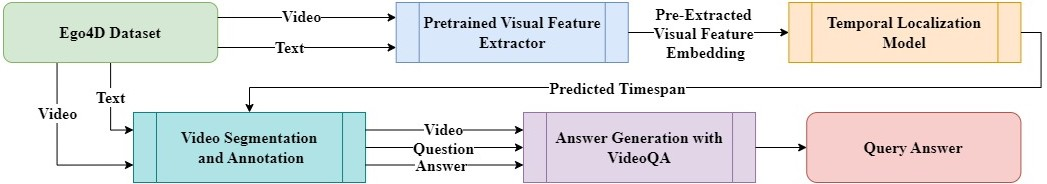
\includegraphics[width=\textwidth]{FullDiagram.jpg}  % Full-page width
		\caption{Pipeline from query-segment prediction to annotation of trimmed clips for VLM input.}
		\label{fig:FullDiagram}
	\end{figure*}
		
We further explore architectural variants of VSLNet, including replacements of the text encoder and encoder-sharing configurations, to assess their effect on localization performance. The most accurate predictions are selected based on mean Intersection over Union (mIoU) scores, and the corresponding video segments are extracted and refined using a two-step ffmpeg-based pipeline. These trimmed clips are manually annotated with textual answers, forming a curated dataset of query-segment-answer triplets. This dataset is used to evaluate the generative capabilities of three advanced Video-Language Models: LLaVA-NeXT, CogVLM2, and InternVideo2.5, each tasked with producing a free-form answer conditioned on the video and query. Model outputs are compared against human references using BLEU and ROUGE metrics, completing an end-to-end framework for grounded answer generation in egocentric video.
	
	
%%%%%%%%%%%%%%%%%%%%%%%%%%%%%%%%%%%%%%%%%%%%%%%%%%%%%%%%%%%%%%%%%%%%
	
	
\subsection{Datasets}
	
We utilize the Ego4D Moments Benchmark dataset\cite{1_Ego4D_Around_the_World_in_3000_Hours_of_Egocentric_Video}, a large-scale, egocentric video corpus consisting of over 3,670 hours of first-person video data collected from 931 unique camera wearers across 74 global locations. The dataset spans a diverse range of unscripted daily-life scenarios such as cooking, commuting, social interactions, and workplace activities. This extensive coverage provides a rich substrate for training and evaluating models on tasks like Natural Language Querying and moment localization.
	
For our work, we focus on a subset of the dataset aligned with the Ego4D Episodic Memory benchmark, where videos are annotated with natural language queries targeting specific temporal segments. This benchmark includes three types of queries: Memory Queries (MQ), Vision Queries (VQ), and Natural Language Queries. We exclusively utilize Natural Language Queries. The dataset structure is as follows:
	\begin{itemize}
		\item[$\bullet$] Each video consists of one or more clips, each with
		defined start and end times.
		\item[$\bullet$] Every clip is annotated by two different individuals,
		ensuring annotation precision and reliability.
		\item[$\bullet$] Each annotation set includes queries and their corre
		sponding timeframes.
	\end{itemize}
	
The NLQ training set which we are using includes 11,291 query-segment instances, with an additional 3,874 instances for validation. Annotations are curated using 13 question templates and cover a wide array of activity contexts, offering strong supervision for video-language localization tasks.
	
To support efficient training, we preprocess these annotations into clip-text pairs. Statistical analysis of the clip durations shows an average length of 522.7 seconds, with a minimum of 207.1 seconds and a maximum of 1200.1 seconds. The standard deviation is 197.6 seconds, and the median clip length is 480 seconds, indicating a moderate variation in activity durations and confirming the dataset’s suitability for temporal reasoning tasks mentioned in Fig.\ref{fig:clip_dist}.
	
	\begin{figure}[htbp]
		\centering
		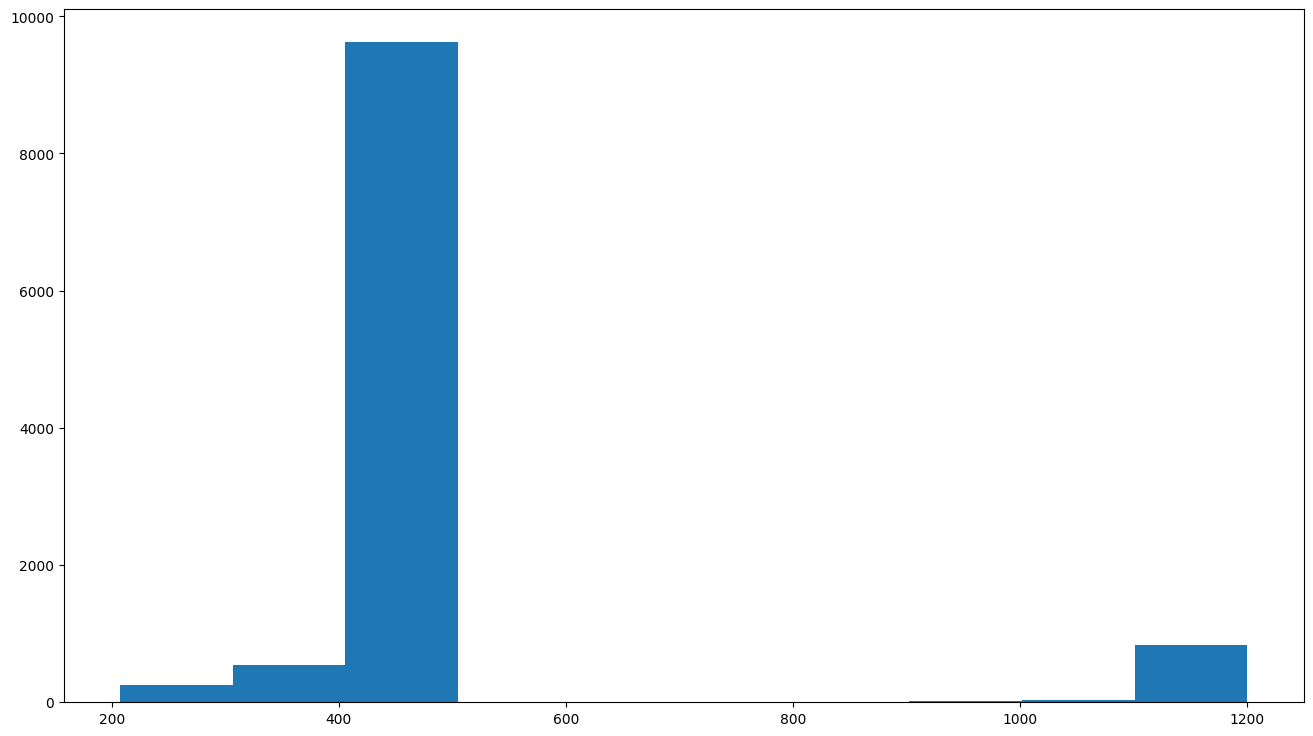
\includegraphics[width=0.8\linewidth]{clip_size_distribution.png}
		\caption{Distribution of clip sizes (in seconds) for NLQ training data.}
		\label{fig:clip_dist}
	\end{figure}
	
We also visualize the distribution of relative query sizes, differentiating between those larger and smaller than 20\% of their parent clip. Fig.\ref{fig:query_gt_0_2} and Fig.\ref{fig:query_lte_0_2} provide insight into how annotation granularity varies with query difficulty or duration. This helps in modeling attention across coarse versus fine temporal spans.
	
	\begin{figure}[htbp]
		\centering
		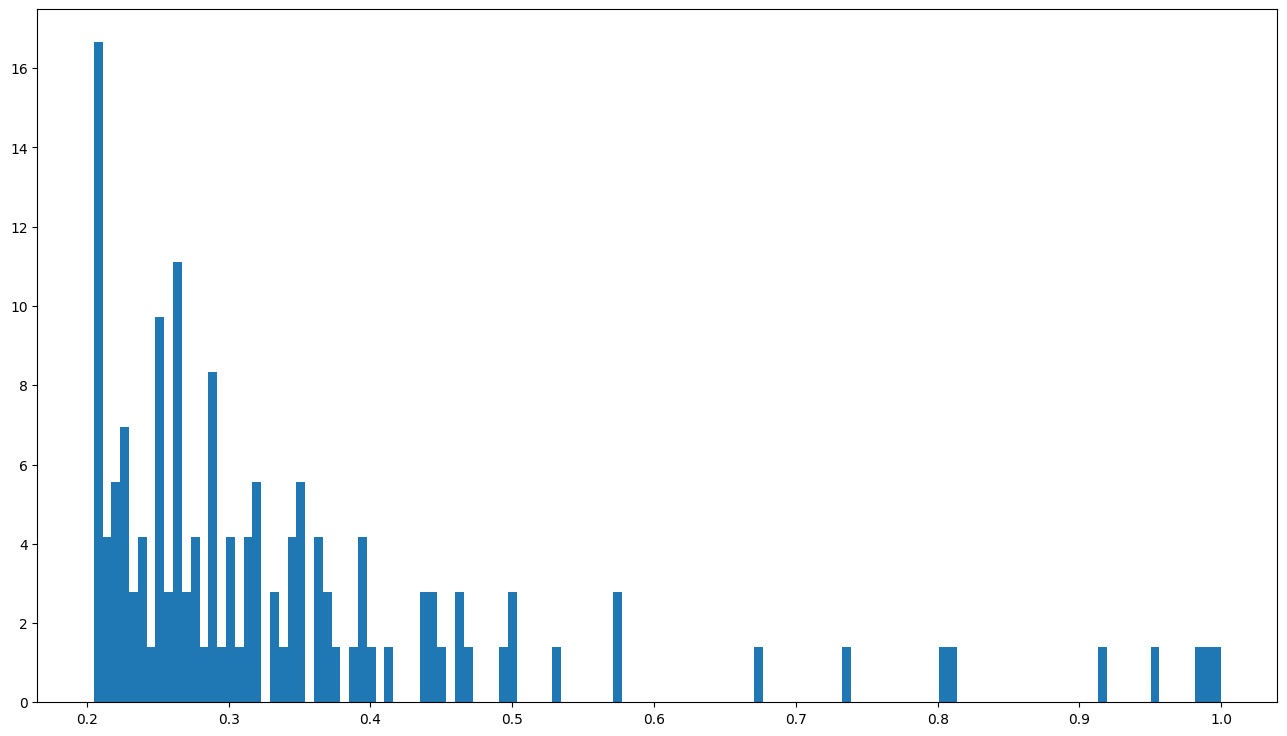
\includegraphics[width=0.8\linewidth]{relative_distribution_of_query_sizes_gt_0_2.png}
		\caption{Distribution of queries where the segment size is $> 20\%$ of the clip.}
		\label{fig:query_gt_0_2}
		
	\end{figure}
	
	\begin{figure}[htbp]
		\centering
		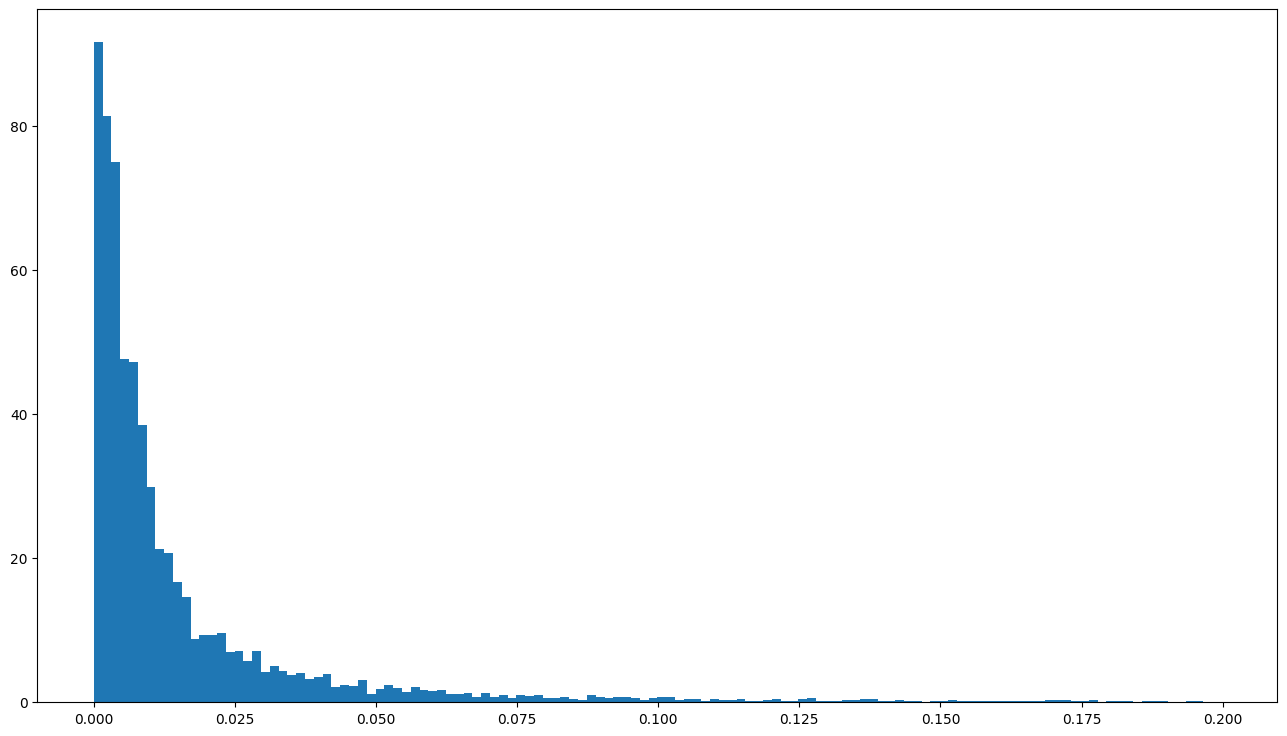
\includegraphics[width=0.8\linewidth]{relative_distribution_of_query_sizes_lte_0_2.png}
		\caption{Distribution of queries where the segment size is $ \leqslant 20\%$ of the clip.}
		\label{fig:query_lte_0_2}
	\end{figure}
	
	
	
%%%%%%%%%%%%%%%%%%%%%%%%%%%%%%%%%%%%%%%%%%%%%%%%%%%%%%%%%%%%%%%%%%%%
	
\subsection{Pre-Extracted Features}
	
	
To effectively address the demands of egocentric video-language tasks, we adopted a transfer learning strategy using pre-extracted features from two complementary models: EgoVLP and Omnivore. EgoVLP, being specifically pretrained on large-scale egocentric video-text data, was particularly aligned with our domain, enabling us to leverage its strong capacity for understanding first-person visual context. This significantly enhanced our model's performance in temporal localization tasks by providing high-quality features tailored to egocentric semantics\cite{6_Egocentric_Video_Language_Pretraining}.
	
In parallel, Omnivore offered a valuable point of comparison. Although not explicitly trained on egocentric data, its generalized architecture, designed to handle multiple visual modalities such as RGB, 3D, and video, allowed us to explore the benefit of broad visual pretraining. Incorporating Omnivore features provided robustness and helped us evaluate the impact of modality-agnostic representations\cite{8_OMNIVORE_ASingle_Model_for_Many_Visual_Modalities}.
	
These two feature extraction models each separately strengthened our system's adaptability and generalization, ultimately supporting more reliable training and evaluation across diverse video-language tasks.
	
%%%%%%%%%%%%%%%%%%%%%%%%%%%%%%%%%%%%%%%%%%%%%%%%%%%%%%%%%%%%%%%%%%%%
	
\subsection{Temporal Localization Models}
\label{sec:temporal}
	
In our experiments, we run both VSLBase and VSLNet in combination with two different feature extraction backbones: Omnivore and EgoVLP, which were discussed in previous sections.
	
VSLBase serves as the core model within the VSLNet framework, built upon a transformer-based architecture that uses self-attention mechanisms to jointly process video and text inputs. By treating the video as a textual passage, VSLBase is designed to predict the start and end boundaries of the answer span within the video stream. It consists of three primary components: a feature encoder, a context-query attention module, and a conditional span predictor. Expanding upon this foundation, VSLNet introduces a Query-Guided Highlighting mechanism, which focuses the model's attention on a relevant region within the video. This highlighted region offers two main advantages: it provides richer contextual information due to the temporal continuity of video, and it reduces the search space, allowing the model to detect finer distinctions between frames. The QGH is implemented through an additional attention layer that dynamically aligns video content with the query. Furthermore, VSLNet includes a contextual multi-head self-attention layer to capture long-range dependencies in the video sequence\cite{4_Span_based_Localizing_Network_for_Natural_Language_Video_Localization}.
	
By pairing each temporal localization model with both feature extractors, we aim to evaluate which combination yields the most accurate results. 

	
%%%%%%%%%%%%%%%%%%%%%%%%%%%%%%%%%%%%%%%%%%%%%%%%%%%%%%%%%%%%%%%%%%%%
	
\subsection{Architectural Variants of VSLNet}
	
To explore the impact of architectural variations in Natural Language Video Localization (NLVL), we extend the original VSLNet model by modifying its text encoding module and encoder sharing scheme. The original VSLNet architecture, as illustrated in Fig.\ref{fig:VSLNet_VSLBase}, employs GloVe embeddings as the text representation and shares a single feature encoder across both video and text modalities.


\begin{figure}[h] % Changed from \begin{figure*}
		\centering
		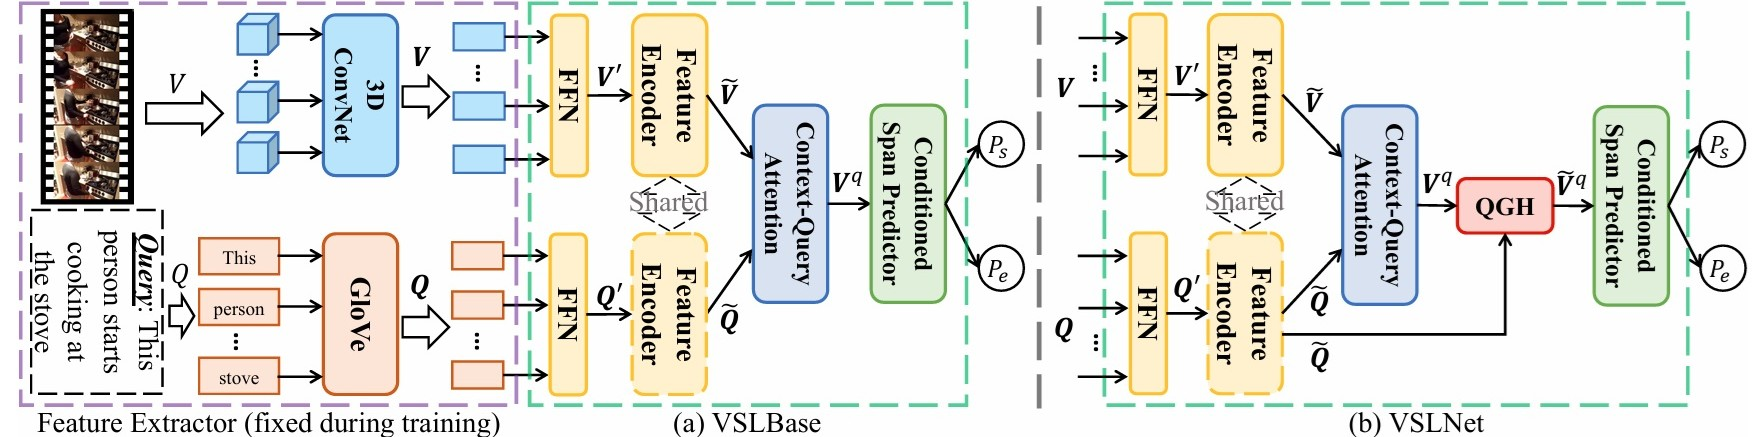
\includegraphics[width=\columnwidth]{VSLNet_VSLBase.jpg} % Changed width=\textwidth to width=\columnwidth
		\caption{The VSLNet architecture, highlighting the dynamic span prediction over video segments \cite{4_Span_based_Localizing_Network_for_Natural_Language_Video_Localization}.}
		\label{fig:VSLNet_VSLBase}
	\end{figure}

	
To address this, we experiment with two key architectural modifications. First, we replace the GloVe-based textual embedding with BERT, a contextualized transformer-based language model, which has demonstrated superior performance in various natural language processing tasks. This change aims to provide richer and more nuanced semantic representations of the language query. Second, we modify the encoder structure by removing the weight-sharing constraint between the visual and textual encoders. In the original design, both modalities are passed through the same encoder with shared parameters. In our variant, we use distinct encoders for video and text features. enabling independent learning paths for each stream, to learn modality-specific transformations. These architectural variants are evaluated in combination with Omnivore and EgoVLP which were discussed earlier to assess their performance across different representation styles. Each configuration is tested independently to identify the optimal pairing of temporal localization model and feature extractor. 
		
%%%%%%%%%%%%%%%%%%%%%%%%%%%%%%%%%%%%%%%%%%%%%%%%%%%%%%%%%%%%%%%%%%%%
		
\subsection{From Temporal Localization to Answer Generation}
	
Building upon the best-performing combination identified in Section \ref{sec:temporal} we extended the task from temporal localization to textual answer generation. The output of the selected NLQ model was used to identify the most accurate predicted segments across the validation set, measured using the mIoU metric over the top five predictions for each query. From this pool, we selected the top 50 queries for which the predicted time spans aligned most closely with ground truth annotations.
	
To extract the relevant visual content from the long-form egocentric videos in the Ego4D dataset, we implemented a two-stage clipping strategy using an automated method with ffmpeg. First, broader video intervals were trimmed based on clip\_uid, which typically included multiple natural language queries. Then, these segments were refined into shorter clips corresponding to individual queries using their specific predicted timestamps. This hierarchical process ensured computational efficiency while retaining semantic precision.
	
To provide supervision for generative answering, we manually annotated each of these clips with a short, accurate textual answer grounded in the visual evidence. This annotation process ensured that the reference answers captured subtle visual cues and context, which are often essential in egocentric video understanding. The full set of annotations and metadata was stored in a structured JSON format that includes the query, predicted and ground truth segments, IoU scores, and the manually created answer for each instance.
	
This dataset serves as input for the next phase, where we evaluate the performance of a Video-Language Model (e.g., Video-LLaVA) on the task of producing free-form answers.
		

	
%%%%%%%%%%%%%%%%%%%%%%%%%%%%%%%%%%%%%%%%%%%%%%%%%%%%%%%%%%%%%%%%%%%%
	
	
\subsection{Answer Generation with VideoQA Models}
	
Following the construction of 50 trimmed and manually annotated egocentric video segments, we advanced to the final step of our pipeline: generating textual answers using Video-Language Models. Each video segment was paired with its corresponding natural language query and served as input to three pretrained VLMs. These models were selected based on their strong performance in video-based inference and were run under consistent conditions using official checkpoints.
	
For each input pair, the models produced a free-form textual answer. These predictions were then evaluated against our manually written reference answers using standard natural language generation metrics. Specifically, we computed BLEU-1, BLEU-2, and BLEU-4 scores to assess n-gram precision, along with ROUGE-1 and ROUGE-L scores to capture content overlap and sequence similarity.
	
This evaluation enables a quantitative comparison of the models’ ability to produce accurate, visually grounded answers based on egocentric video content. The results are analyzed in detail in the following section.
	
	
%%%%%%%%%%%%%%%%%%%%%%%%%%%%%%%%%%%%%%%%%%%%%%%%%%%%%%%%%%%%%%%%%%%%%%%%	
\section{Experiments and results}

We evaluate our pipeline across two core tasks: temporal localization and answer generation for egocentric video. Models are assessed using standard metrics, Recall@k with IoU for localization, and BLEU and ROUGE for generation. Results highlight the impact of feature extractors, model variants, and domain alignment. Quantitative findings are complemented by qualitative examples, offering insight into model grounding and answer fidelity.
	
%%%%%%%%%%%%%%%%%%%%%%%%%%%%%%%%%%%%%%%%%%%%%%%%%%%%%%%%%%%%%%%%%%%%%%%%	

\subsection{Training Parameters}

To ensure consistency and fairness across experimental comparisons, we retained the default hyperparameter configurations for all models evaluated in this study. For both VSLNet and VSLBase, we used the official training presets: batch size of 32, hidden dimension of 128, maximum sequence length of 128, initial learning rate of 0.0025, and 10 training epochs. These hyperparameters, empirically validated in the original work, provided a balanced trade-off between training stability and computational efficiency. Likewise, for the video-language models used during the answer generation stage we adhered to their default inference settings as reported by the authors in their respective publications[reference to LLaVA-NEXT article] or huggingface and github repositories.
For instance, LLaVA-NeXT was executed with top-p sampling (0.9), a limit of 100 new tokens, and enabled sampling mode; CogVLM2 used a larger decoding window with 2048 new tokens and a low-temperature greedy decoding strategy; InternVideo2.5 was configured with a maximum of 512 frames, 128 segments, and deterministic decoding with temperature set to zero. Maintaining default hyperparameters allowed us to isolate the impact of feature encoders and localization architectures without introducing additional optimization bias, thereby preserving the reproducibility and integrity of our results.


	
%%%%%%%%%%%%%%%%%%%%%%%%%%%%%%%%%%%%%%%%%%%%%%%%%%%%%%%%%%%%%%%%%%%%%%%%	
	
\subsection{Intersection over Union}
	
To evaluate the performance of different combinations of models and feature extractors, we use the Intersection over Union metric as the principal measure of temporal localization accuracy. Formally, IoU is defined as shown in Equation \eqref{eq:iou_formula}.		
	\begin{equation}
		IoU = \frac{| \text{Predicted Segment} \cap \text{Ground Truth Segment} |}{| \text{Predicted Segment} \cup \text{Ground Truth Segment} |}
		\label{eq:iou_formula} % Add a label here. You can choose any unique name.
	\end{equation}		 
where the numerator denotes the duration of the overlap between the predicted and ground-truth segments, and the denominator captures the total span covered by either. A higher IoU reflects more precise temporal alignment. We evaluate model performance using Recall@1 and Recall@5 at two IoU thresholds (0.3 and 0.5), where Recall@k indicates the proportion of queries for which at least one of the top-k predicted segments exceeds the specified IoU threshold. This multi-level evaluation enables a robust comparison of localization fidelity across model architectures, feature encoders, and design variants.
	
	
%%%%%%%%%%%%%%%%%%%%%%%%%%%%%%%%%%%%%%%%%%%%%%%%%%%%%%%%%%%%%%%%%%%%%%%%		
\subsection{Temporal Localization Performance}
	
Table \ref{tab:net_base} compares the performance of VSLNet and VSLBase across Omnivore and EgoVLP features, evaluated on the Ego4D NLQ task using Recall@1 and Recall@5 at IoU thresholds of 0.3 and 0.5. The results clearly show that VSLBase combined with EgoVLP features yields the strongest overall performance, achieving 7.82\% Recall@1 and 15.18\% Recall@5 at IoU 0.3, and 5.01\% Recall@1 and 10.20\% Recall@5 at IoU 0.5.
Notably, when using EgoVLP, VSLBase consistently outperforms VSLNet across all metrics, indicating that the simpler span-based architecture benefits more directly from the semantically aligned and egocentrically pretrained features of EgoVLP. In contrast, when paired with Omnivore, VSLNet slightly outperforms VSLBase at IoU 0.3 Recall@1, but this advantage diminishes at higher thresholds. This suggests that VSLNet’s Query-Guided Highlighting (QGH) may offer a marginal benefit when feature representations are less well aligned with language, as in the case of Omnivore.
Across all configurations, the official Ego4D baseline, which uses VSLNet with Omnivore, exhibits the weakest results, reinforcing the importance of using domain-specific feature encoders in egocentric tasks. Overall, the results highlight that the most effective combination for temporal localization is VSLBase with EgoVLP features, striking a strong balance between architectural efficiency and high-quality visual representation.
	
		\begin{table}[h!]
		\small
		\setlength{\tabcolsep}{3pt}
		\centering
		% Increase row height (1.8 is larger than the default 1)
		\renewcommand{\arraystretch}{1.98}
		\begin{tabularx}{\linewidth}{|c|c|C|C|C|C|} % Changed to tabularx and using 'C' for auto-width centered columns
			\hline
			\multirow{2}{*}{\rotatebox[origin=c]{90}{Dataset}} & \multirow{2}{*}{\textbf{Model}} & \multicolumn{2}{c|}{\textbf{IoU=0.3(\%)}} & \multicolumn{2}{c|}{\textbf{IoU=0.5(\%)}} \\  \cline{3-6}
			
			&   & \textbf{r@1}& \textbf{r@5} & \textbf{r@1}& \textbf{r@5} \\ \hline
			\multirow{2}{*}{\rotatebox[origin=c]{90}{Omnivore}}
			& VSLNet & 6.659 & 13.5261 & 3.536 & 8.260 \\ \cline{2-6}
			& VSLBase & 6.427 & 13.216 & 3.639 & 8.776 \\ \hline
			\multirow{2}{*}{\rotatebox[origin=c]{90}{EgoVLP}}
			& VSLNet & 6.814 & 14.300 & 4.104 & 9.525 \\ \cline{2-6}
			& VSLBase & \textbf{7.821} & \textbf{15.178} & \textbf{5.007} & \textbf{10.196} \\ \hline
			\multicolumn{2}{|c|}{Baseline \cite{5_SlowFast_Networks_for_Video_Recognition}} & 5.45 & 10.74 & 3.12 & 6.63 \\ \hline
		\end{tabularx} % Changed from tabular
		
		% Add vertical space between table and caption
		\vspace{0.5em}
		
		\caption{Comparison of VSLNet and VSLBase Performance Using Omnivore and EgoVLP Features Against Official Ego4D Baseline \cite{1_Ego4D_Around_the_World_in_3000_Hours_of_Egocentric_Video}. The results of VSLBase on EgoVLP dataset proves better performance among all the combinations.}
		\label{tab:net_base}
	\end{table}
	
%%%%%%%%%%%%%%%%%%%%%%%%%%%%%%%%%%%%%%%%%%%%%%%%%%%%%%%%%%%%%%%%%%

\subsection{Evaluation of VSLNet Variants}

Table~\ref{tab:Glove_NSE} presents the performance comparison of two architectural variants of VSLNet: one using GloVe embeddings with a shared encoder, and the other using non-shared encoders with BERT embeddings. As before, these models were evaluated using visual features extracted from both Omnivore and EgoVLP. The results are reported using Recall@1 and Recall@5 at IoU thresholds of 0.3 and 0.5, consistent with our previous evaluation methodology.
Across all settings, the NSE variant combined with EgoVLP features achieves the highest scores, with Recall@1 and Recall@5 reaching 8.93\% and 16.65\% at IoU 0.3, and 5.42\% and 11.18\% at IoU 0.5. This improvement validates our hypothesis that separating the video and text encoders enables more specialized modality-specific representation learning, which enhances temporal localization performance. Moreover, replacing GloVe with BERT allows the model to capture richer and contextually grounded semantics in natural language queries, which is particularly beneficial in egocentric settings where queries often refer to subtle, temporally dispersed visual cues.
The performance gain is most pronounced when using EgoVLP features, which are already semantically aligned through egocentric video-language pretraining. This suggests that the architectural enhancements introduced in the NSE variant amplify the benefits of high-quality visual representations. In contrast, the improvements are less substantial when paired with Omnivore, a domain-agnostic visual backbone. This indicates that the gains from NSE architecture are most effective when the input features are already closely aligned with language semantics, as is the case with EgoVLP.
Overall, these findings highlight the compounding effect of modality-specific encoders and domain-specific visual features in improving moment localization performance. The superior performance of the NSE + EgoVLP combination further supports the importance of fine-grained visual-language alignment in egocentric video understanding.
	
		
	\begin{table}[h!]
		\centering
		% Increase row height (1.8 is larger than the default 1)
		\renewcommand{\arraystretch}{1.98}
		\begin{tabularx}{\linewidth}{|c|c|C|C|C|C|} % Changed to tabularx and using 'C' for auto-width centered columns
			\hline
			\multirow{2}{*}{\rotatebox[origin=c]{90}{Dataset}} & \multirow{2}{*}{\textbf{Model}} & \multicolumn{2}{c|}{\textbf{IoU=0.3(\%)}} & \multicolumn{2}{c|}{\textbf{IoU=0.5(\%)}} \\  \cline{3-6}
			
			&   & \textbf{r@1}& \textbf{r@5} & \textbf{r@1}& \textbf{r@5} \\ \hline
			\multirow{2}{*}{\rotatebox[origin=c]{90}{Omnivore}}
			& Glove & 2.813 & 7.614 & 1.316 & 3.897 \\ \cline{2-6}
			& NSE & 5.756 & 12.106 & 2.839 & 7.563 \\ \hline
			\multirow{2}{*}{\rotatebox[origin=c]{90}{EgoVLP}}
			& Glove & 6.556 & 13.113 & 3.872 & 8.673\\ \cline{2-6}
			& NSE & \textbf{8.931} & \textbf{16.649} & \textbf{5.420} & \textbf{11.177} \\ \hline
			
		\end{tabularx} % Changed from tabular
		
		% Add vertical space between table and caption
		\vspace{0.5em}
		
		\caption{Evaluation of VSLNet variants with different encoder configurations—GloVe and Non-Shared Encoders—across Omnivore and EgoVLP datasets. The results of NSE on EgoVLP dataset demonstrate higher scores compared to other experiments.}
		\label{tab:Glove_NSE}
	\end{table}
	


%%%%%%%%%%%%%%%%%%%%%%%%%%%%%%%%%%%%%%%%%%%%%%%%%%%%%%%%%%%%%%%%%%%%%%%%	
	
\subsection{NLP Metrics for Answer Generation}

To assess the quality of generated textual answers in our VideoQA pipeline, we employ BLEU and ROUGE, two well-established metrics in natural language generation. These metrics evaluate how closely a model-generated answer matches the human-annotated reference answer, offering complementary perspectives.

\textbf{$\bullet$ BLEU (BLEU-1, BLEU-2, BLEU-4):}

BLEU, or Bilingual Evaluation Understudy, evaluates n-gram overlap between the candidate and reference answers. It calculates how many contiguous sequences of tokens in the generated text are also present in the reference. BLEU-1 focuses on unigrams and provides a basic measure of lexical similarity, capturing whether the right words are used. BLEU-2 extends this to bigrams, introducing a sensitivity to word pairing and local grammatical structure. BLEU-4 considers up to four-gram sequences, offering a more stringent measure that rewards coherent phrasing and syntactic fluency. Higher-order BLEU scores tend to better reflect human judgments of naturalness, especially for longer answers.

\textbf{$\bullet$ ROUGE (ROUGE-1, ROUGE-L):}

ROUGE, or Recall-Oriented Understudy for Gisting Evaluation, is recall-based and evaluates how much of the reference answer is recovered by the generated response. ROUGE-1 measures unigram recall, assessing whether the key content words from the reference appear in the candidate answer. ROUGE-L is based on the longest common subsequence between the two texts and captures not only content overlap but also word order and structural similarity. It is especially useful for tasks that value fluent, human-like sentence construction.

The combination of BLEU and ROUGE provides a robust evaluation framework across multiple dimensions for open-ended answer generation in egocentric video understanding.
	
	
%%%%%%%%%%%%%%%%%%%%%%%%%%%%%%%%%%%%%%%%%%%%%%%%%%%%%%%%%%%%%%%%%%%%%%%%	
	
\subsection{Generative Answering Results}


Table~\ref{tab:vlms_performance} presents the BLEU and ROUGE scores for the three Video-Language Models evaluated on the task of answer generation from egocentric video-query pairs: LLaVA-NeXT, CogVLM2, and InternVideo2.5. Each model was provided with a manually curated dataset of 50 trimmed video clips paired with natural language queries, and tasked with producing short, grounded textual answers. The outputs were quantitatively assessed against human-written references using BLEU-1, BLEU-2, and BLEU-4 for n-gram precision, and ROUGE-1 and ROUGE-L for content recall and structural alignment.

Among the three models, InternVideo2.5 achieved the highest performance across all metrics, with BLEU-1 of 0.2327, BLEU-2 of 0.1694, and BLEU-4 of 0.0961, as well as ROUGE-1 and ROUGE-L scores of 0.4633 and 0.4149 respectively. These results reflect a strong capacity for both lexical accuracy and sequence-level fluency. This superior performance can be attributed to InternVideo2.5’s design, which incorporates long-context modeling, hierarchical token merging, and dense vision-language alignment. Such mechanisms enable it to process extended video segments more effectively, preserving fine-grained semantic cues crucial for answering open-ended egocentric questions.

CogVLM2 ranks second, showing competitive performance with BLEU-1 of 0.2271 and ROUGE-L of 0.3085. While it benefits from timestamp-aware vision-language fusion and robust grounding capabilities, its relatively shorter decoding window and less aggressive frame selection compared to InternVideo2.5 may limit its capacity to aggregate broader visual context in egocentric video segments.

LLaVA-NeXT demonstrates the weakest performance across all metrics. With a BLEU-1 of 0.1229 and ROUGE-L of 0.1805, it struggles to produce precise or structurally coherent answers. Despite its instruction-tuned design and multi-modal capability, its reliance on sparsely sampled visual frames and generalized training data may reduce its effectiveness in densely grounded, context-rich egocentric scenarios.

Overall, these results validate the importance of temporal context modeling, dense vision-language fusion, and frame-level granularity in VideoQA tasks. InternVideo2.5's performance underscores the need for architectures that are not only capable of visual reasoning but also optimized for long-form egocentric content.

	
	\begin{table}[ht]
		\small  % Reduce font size
		\setlength{\tabcolsep}{4pt}  % Reduce horizontal spacing between columns
		\centering
		\begin{tabular}{lccccc}
			\toprule
			\textbf{Model} & \textbf{B-1} & \textbf{B-2} & \textbf{B-4} & \textbf{R-1} & \textbf{R-L} \\
			\midrule
			LLaVA-NeXT      & 0.1229 & 0.0645 & 0.0246 & 0.2313 & 0.1805 \\
			CogVLM2         & 0.2271 & 0.1593 & 0.0795 & 0.3660 & 0.3085 \\
			InternVideo2.5  & \textbf{0.2327} & \textbf{0.1694} & \textbf{0.0961} & \textbf{0.4633} & \textbf{0.4149} \\
			\bottomrule
		\end{tabular}
		\caption{BLEU and ROUGE scores of evaluated VLMs.}
		\label{tab:vlms_performance}
	\end{table}
	
	
%%%%%%%%%%%%%%%%%%%%%%%%%%%%%%%%%%%%%%%%%%%%%%%%%%%%%%%%%%%%%%%%%%%%%%%%	
	
	
\subsection{Qualitative Examples}

To complement our quantitative evaluation, we conduct a qualitative analysis of the answers produced by the three evaluated Video-Language Models on a representative query from the Ego4D dataset. Fig.\ref{fig:VLMs_Qualitative} illustrates a frame from an egocentric video clip alongside the corresponding natural language query, ground-truth answer, and the generated outputs of each model.
The query, “what tool did I sharpen the pencils with?”, refers to a concrete, visually grounded action captured from a first-person perspective. The ground-truth answer correctly identifies the tool as a “utility knife (box cutter),” as evidenced by the subject’s hands holding and using a red utility knife in the video frame.
Among the model outputs, InternVideo2.5 provides the most semantically accurate response, stating that “you sharpened the pencils with a green utility knife.” Despite the minor error in color attribution (“green” instead of red), the model correctly identifies both the tool type and the action, demonstrating effective visual grounding and object recognition. This aligns with the model’s strong quantitative performance and reflects its architectural emphasis on long-context video modeling and fine-grained visual-text alignment.
CogVLM2, by contrast, produces a hallucinated response: “The man used a wood chisel to sharpen the pencils.” This answer incorrectly identifies the tool and introduces an ungrounded gender attribution, despite the query being framed in the first person. The hallucination suggests an over-reliance on generic language priors rather than visual evidence, potentially due to weaker object-level grounding under egocentric conditions.
LLaVA-NeXT also fails to correctly identify the tool, instead describing it as a “manual pencil sharpener.” While the description reflects a plausible sharpening mechanism, it lacks correspondence with the visual scene, indicating limited visual grounding in high-resolution egocentric frames. This is consistent with the model’s lower quantitative scores and suggests challenges in visual-text alignment when pretraining is not domain-specific.
Overall, the qualitative results reinforce our quantitative findings and emphasize the critical role of domain alignment and temporal context modeling in producing accurate, visually grounded answers in first-person video settings.
	\begin{figure}[h] % Changed from \begin{figure*}
			\centering
			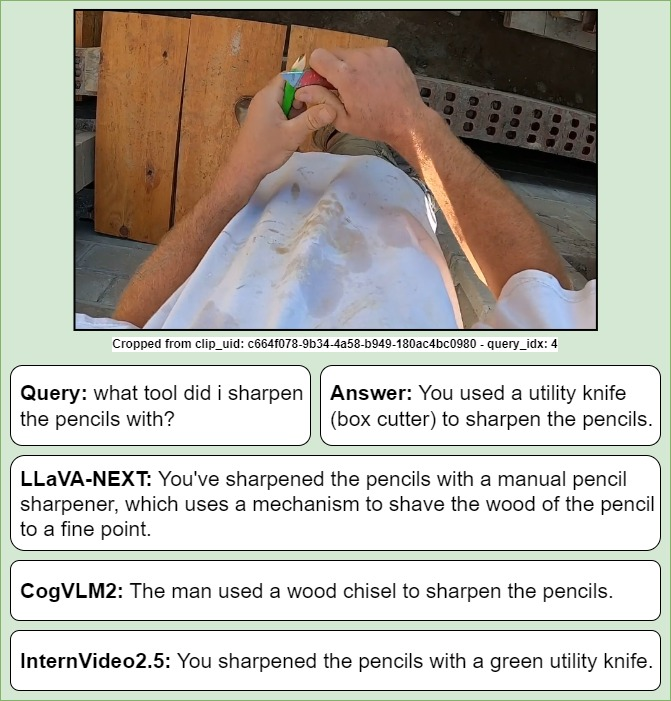
\includegraphics[width=\columnwidth]{VLMs_Qualitative.jpg} % Changed width=\textwidth to width=\columnwidth
			\caption{Qualitative comparison of answers generated by LLaVA-NeXT, CogVLM2, and InternVideo2.5 for a representative egocentric clip from the Ego4D dataset.}
			\label{fig:VLMs_Qualitative}
		\end{figure}
	
%%%%%%%%%%%%%%%%%%%%%%%%%%%%%%%%%%%%%%%%%%%%%%%%%%%%%%%%%%%%%%%%%%
	
\section{Discussions and findings}
	
	
In this project, we tackled the complex task of answering natural language queries on egocentric videos through a unified two-stage pipeline. Our work began with the temporal localization of relevant video segments using span-based models and evolved into the evaluation of answer generation using state-of-the-art Vision-Language Models.
Through comprehensive experimentation, we showed that VSLNet consistently outperforms the lighter VSLBase model, especially when paired with EgoVLP features. Furthermore, the use of Non-Shared Encoders proved to be an effective architectural enhancement, significantly improving localization accuracy by better aligning the modalities of video and language.
In the second stage of our pipeline, we introduced an evaluation of three advanced VLMs on a curated set of top 50 query-segment pairs. InternVideo2.5 demonstrated superior performance across both quantitative metrics (BLEU, ROUGE) and qualitative assessments, highlighting its strength in modeling temporal context and producing more accurate answers.
Overall, our findings reinforce the importance of modality-specific features and architectural flexibility in NLQ tasks, especially within the egocentric vision domain. By extending traditional temporal grounding models with answer generation capabilities, we offer a holistic framework that not only finds the right moment but also communicates what happens in that moment. This pipeline paves the way for more intelligent, interactive systems capable of understanding and summarizing human experiences from first-person perspectives.
	
%%%%%%%%%%%%%%%%%%%%%%%%%%%%%%%%%%%%%%%%%%%%%%%%%%%%%%%%%%%%%%%%%%%%%%%%	 
\section{Acknowledgements}

The acknowledgements express sincere gratitude to the course instructors and teaching assistants of the Machine Learning and Deep Learning course at Politecnico di Torino for their continuous guidance and support, which significantly shaped the research direction. Thanks are also extended to the maintainers of the Ego4D benchmark and the open-source communities of VSLNet, CogVLM2, LLaVA, and InternVideo2.5, whose contributions facilitated the experimental pipeline.
	
%%%%%%%%% REFERENCES

	{\small
		\bibliographystyle{ieee_fullname}
		\bibliography{egbib}
	}
	
\end{document}